% ============================================================
%  Two motor items as a candidate cross-context suggestibility screener
%  Compile: pdflatex preprint && bibtex preprint && pdflatex preprint && pdflatex preprint
% ============================================================
\documentclass[12pt,a4paper]{article}

\usepackage[margin=2.5cm]{geometry}
\usepackage{setspace}
\usepackage{graphicx}
\usepackage{booktabs}
\usepackage{amsmath}
\usepackage{amssymb}
\usepackage{natbib}
\usepackage{hyperref}
\usepackage[expansion=false]{microtype}
\usepackage{array}
\usepackage{multirow}
\usepackage{xcolor}
\usepackage{caption}

\hypersetup{colorlinks=true, linkcolor=blue!60!black,
            citecolor=blue!60!black, urlcolor=blue!60!black}

\doublespacing

\begin{document}

% ---- Title page ----
\begin{titlepage}
  \vspace*{2cm}
  \begin{center}
    {\LARGE\bfseries Two motor-challenge items as a candidate\\[6pt]
    cross-context suggestibility screener}\\[2em]
    {\large W.\ Weaver}\\[3em]
    {\normalsize
      Word count: $\approx$4{,}200 \quad Figures: 5 \quad Tables: 4
    }\\[3em]
    \hrule\vspace{1em}
    {\small\textit{Secondary reanalysis of publicly available data.
    Not preregistered. No conflicts of interest. No funding.}}
  \end{center}
\end{titlepage}

% ---- Abstract ----
\begin{abstract}
\noindent
Full suggestibility assessment is often impractical in screening contexts.
We asked whether two motor-challenge items---arm rigidity and arm
immobilisation---show enough cross-context validity to motivate a standalone
first-pass screener.
Applying a consistent analysis to five open datasets ($N = 240$--$584$)
spanning non-hypnotic (PCS), hypnotic (SWASH), and classic group-administered
(HGSHS:A) contexts, the motor composite correlated $r = 0.78$--$0.85$ with
the full-scale total (intensity and involuntariness scales; $r = 0.68$ on
the objective binary) and $r = 0.55$--$0.69$ with the remaining non-motor
items (overlap-free). Music hallucination and negative visual hallucination
approach floor in unselected samples (80--93\% at zero); with near-universal
zero scores they add little to between-person variance on the total, which
is therefore disproportionately shaped by higher-variance challenge items. Classification
weighted $\kappa$ ranged $0.50$--$0.55$ (PCS) and $0.65$ (SWASH and
HGSHS:A involuntariness) against the full total, and $0.29$--$0.52$ against
the overlap-free rest score. Against external criteria with no item overlap,
the motor pair retained 71--80\% of the full scale's predictive signal.
The pattern holds across contexts and measurement axes. These results
support prospective validation of the motor pair as a standalone first-pass
screener in unselected samples.
\end{abstract}

\noindent\textbf{Keywords:} hypnotic suggestibility; phenomenological control;
SWASH; PCS; HGSHS:A; short form; screening; floor effects

\clearpage

% ============================================================
\section{Introduction}

Full administration of standard suggestibility scales---PCS \citep{lush2021pcs},
SWASH \citep{lush2018swash}, HGSHS:A \citep{shor1962hgshs}---requires
ten or more suggestion items, structured administration, and per-item
ratings. For screening, online intake, or time-limited contexts, this is
often not feasible.

Whether such administration is necessary depends on where between-person
variance actually concentrates. A long-standing critique observes that item
difficulty is uneven: several suggestions are passed by very few people
in unselected samples and therefore carry little discriminating information
\citep{coe1971difficulty, sadler2004irt}. Bifactor analysis of HGSHS:A supports a general factor structure with
minor domain-specific components \citep{zahedi2022bifactor}, though whether
a unitary general factor underlies suggestibility scales more broadly remains
an open question. Principal component analysis of the normative PCS and SWASH
data shows a consistent first-component structure within those scales
\citep[supplementary materials]{lush2021pcs}: the motor pair (arm rigidity,
arm immobilisation) loads most strongly on the first component in both
conditions (PCS: 0.706--0.727; SWASH: 0.782--0.803), while music
hallucination and negative visual hallucination load weakly (0.19--0.41
in PCS), consistent with their near-floor rates. On the second component,
passive ideomotor items (hand lowering, hands together) and perceptual
items (mosquito, visual hallucination) occupy opposite poles; the motor
challenge items sit between them, near-neutral on this dimension---especially
under induction, where arm rigidity loads $-0.05$ on PC2. The motor pair is
structurally central: highest on the first component, minimally pulled toward
either secondary pole, and consistent with indexing a broad shared factor
if one exists.

If variance concentrates in the motor pair, a two-item composite may
serve as a first-pass screener. A motor-focused five-item short form of
HGSHS:A achieves $r = 0.83$ and $\kappa \approx 0.58$ against its parent
\citep{riegel2021hgshs5g, zech2024hgshs5g}. What has not been examined
is whether a similar structure holds across hypnotic and non-hypnotic
contexts, across intensity vs.\ involuntariness measurement axes, and whether
a two-item composite produces defensible classification metrics.

We apply a consistent pipeline to five open datasets spanning all three
contexts. We report part-whole and overlap-free correlations, classification
metrics, an all-pairs comparison, external validity tests, and retest
stability. The motor pair items are arm rigidity and arm immobilisation:
mid-scale in unselected samples, high variance, behaviourally observable.


% ============================================================
\section{Method}

\subsection{Datasets}

Five open datasets were analysed (Table~\ref{tab:datasets}). PCS and SWASH
use identical ten-item suggestion sets rated 0--5 for subjective intensity;
they differ only in administration context. HGSHS:A uses the Bowers Involuntariness Scale
\citep{bowers1981suggestion} (0 = did not experience; 1 = voluntary;
5 = involuntary-automatic) and objective pass/fail; it
is analysed separately and never pooled with the intensity datasets.
Dataset-provided exclusion variables were applied, removing $n = 6$
participants from the Norms sample, $n = 18$ from the HGSHS:A sample, and
$n = 62$ from the vEAR-PCS sample. The SWASH validation sample was
additionally restricted to participants with non-missing first-test scores
($n = 77$ excluded).

\begin{table}[ht]
\centering
\caption{Dataset summary.}
\label{tab:datasets}
\footnotesize
\begin{tabular}{llllrr}
\toprule
Sample & Scale & Context & Dimension & $N_{\text{raw}}$ & $N_{\text{analytic}}$ \\
\midrule
Norms-PCS   & PCS     & Non-hypnotic  & Intensity   & 490 & 244 \\
Norms-SWASH & SWASH   & Hypnotic      & Intensity   & 490 & 240 \\
PCS-VVIQ    & PCS     & Non-hypnotic  & Intensity   & 508 & 508 \\
SWASH-val   & SWASH   & Hypnotic      & Intensity   & 495 & 418 \\
HGSHS:A     & HGSHS:A & Classic group & Inv.+Obj.   & 602 & 584 \\
vEAR-PCS    & PCS     & Non-hypnotic  & Intensity   & 514 & 452 \\
\bottomrule
\multicolumn{6}{l}{\parbox{11cm}{\textit{Note.} Norms sample: participants randomly assigned to PCS or SWASH condition; each participant contributed to one condition. OSF accession codes in Open Science Statement.}}\\
\end{tabular}
\end{table}

\subsection{Scoring}

Author-precomputed totals were used for the Norms, SWASH validation, and
vEAR-PCS samples. For the PCS-VVIQ sample, the canonical 10-item mean was
computed with geometric-mean post-hypnotic suggestion
($\sqrt{\text{urge} \times \text{amnesia}}$) and arithmetic-mean taste.

The motor composite is the sum of the arm rigidity and arm immobilisation
items. Source column names: Norms sample: \texttt{ArmRigidity\-Subjective\-Rating}
+ \texttt{ArmImmobilisation\-Subjective\-Rating}; PCS-VVIQ and vEAR-PCS samples:
\texttt{StiffArm} + \texttt{HandAndArmHeavy}; SWASH validation sample:
\texttt{Q5RIGIDITYSUBJ} + \texttt{Q6IMMOBILESUBJ}; HGSHS:A sample:
\texttt{INV.6} + \texttt{INV.4} (involuntariness) or \texttt{HGSHS.A6} +
\texttt{HGSHS.A4} (objective).

\subsection{Analyses}

Two correlation metrics are reported per dataset: $r_{\text{full}}$ (motor
composite vs.\ full-scale total; motor items inside the total) and
$r_{\text{rest}}$ (motor composite vs.\ the remaining non-motor items, no
shared items). Both are always reported together. Sum and mean scoring are linear transforms and produce identical
correlations. Itemwise z-scored composites were checked as a sensitivity
analysis and produced materially unchanged results. Listwise deletion
changes nothing. Spearman-Brown reliability $= 2r/(1+r)$, where $r$ is
the inter-item correlation \citep{eisinga2013spearman}. All CIs are 95\%
bootstrap ($n_{\text{boot}} = 5000$, seed\,=\,20260603).

Classification used tertile groups (low/medium/high) with weighted Cohen's
$\kappa$ (linear weights). Both the full-scale total and the overlap-free
rest score are reported as criteria; the latter quantifies classification
agreement not attributable to shared items. Binary cutoff sweeps (8\%--33\%)
provide AUC, sensitivity, specificity, PPV, and NPV. All-pairs analysis computed $r_{\text{full}}$ and $r_{\text{rest}}$ for all
$\binom{10}{2} = 45$ two-item combinations in the PCS/SWASH-style 10-item
samples. External validity tested motor pair vs.\
full scale against five criteria with no item overlap with the PCS.


% ============================================================
\section{Results}

\subsection{Convergence}

The Norms sample provides the cleanest context comparison: participants were
randomly assigned to PCS or SWASH from a common pool, so the correlation
difference is attributable to the administered context---including hypnotic
induction and associated framing---rather than cohort differences. Motor composite
correlations were higher under SWASH ($r_{\text{full}} = 0.849$,
$r_{\text{rest}} = 0.694$) than PCS ($r_{\text{full}} = 0.783$,
$r_{\text{rest}} = 0.565$); Fisher's $r$-to-$z$ confirms the difference
($r_{\text{full}}$: $z = -2.18$, $p = .029$; $r_{\text{rest}}$: $z = -2.36$,
$p = .018$). Hypnotic induction amplifies the motor-pair coupling; both
contexts produce substantial correlations.

Table~\ref{tab:convergence} and Figure~\ref{fig:forest} show the full
pattern. Across three PCS datasets, the motor composite correlated
$r_{\text{full}} = 0.78$--$0.79$ ($R^2 = 0.61$--$0.62$) and
$r_{\text{rest}} = 0.55$--$0.58$, replicating tightly across independent
cohorts ($N = 244$--$508$). SWASH shows higher coupling: $r_{\text{full}} =
0.81$--$0.85$, $r_{\text{rest}} = 0.63$--$0.69$. Cross-dataset PCS--SWASH
comparisons are non-significant ($p = .24$, $.38$), consistent with
between-cohort variability dominating in separate samples. HGSHS:A
involuntariness falls between ($r_{\text{full}} = 0.80$, $r_{\text{rest}} =
0.66$). HGSHS:A objective binary is lower ($r_{\text{full}} = 0.68$),
consistent with binary scoring discarding within-item variation.

\begin{table}[ht]
\centering
\caption{Motor composite correlations with full-scale total and rest score.}
\label{tab:convergence}
\small
\begin{tabular}{lrrrrrrr}
\toprule
Sample & $N$ & $r_{\text{full}}$ & $R^2$ & 95\% CI & $r_{\text{rest}}$ & 95\% CI & SB \\
\midrule
Norms-PCS      & 244 & 0.783 & 0.61 & [0.732, 0.827] & 0.565 & [0.474, 0.644] & 0.61 \\
PCS-VVIQ       & 508 & 0.778 & 0.61 & [0.741, 0.811] & 0.549 & [0.483, 0.612] & 0.63 \\
vEAR-PCS       & 452 & 0.785 & 0.62 & [0.748, 0.819] & 0.579 & [0.514, 0.641] & 0.62 \\
\midrule
Norms-SWASH    & 240 & 0.849 & 0.72 & [0.814, 0.880] & 0.694 & [0.624, 0.754] & 0.79 \\
SWASH-val      & 418 & 0.807 & 0.65 & [0.774, 0.838] & 0.630 & [0.570, 0.687] & 0.75 \\
\midrule
HGSHS:A (inv.) & 584 & 0.799 & 0.64 & [0.768, 0.827] & 0.659 & [0.610, 0.705] & 0.70 \\
HGSHS:A (obj.) & 584 & 0.682 & 0.46 & [0.639, 0.720] & 0.449 & [0.384, 0.511] & 0.42 \\
\midrule
\textit{HGSHS-5:G (prior short form)} & --- & \textit{0.83} & \textit{0.69} & --- & --- & --- & --- \\
\bottomrule
\multicolumn{8}{l}{\parbox{14cm}{\textit{Note.} $r_{\text{full}}$: motor items inside total. $r_{\text{rest}}$: motor pair vs.\ non-motor rest score. SB: Spearman-Brown reliability. CIs: 95\% bootstrap ($n_{\text{boot}} = 5000$). All $p < .001$. HGSHS-5:G: \citet{riegel2021hgshs5g, zech2024hgshs5g}.}}\\
\end{tabular}
\end{table}

\begin{figure}[ht]
\centering
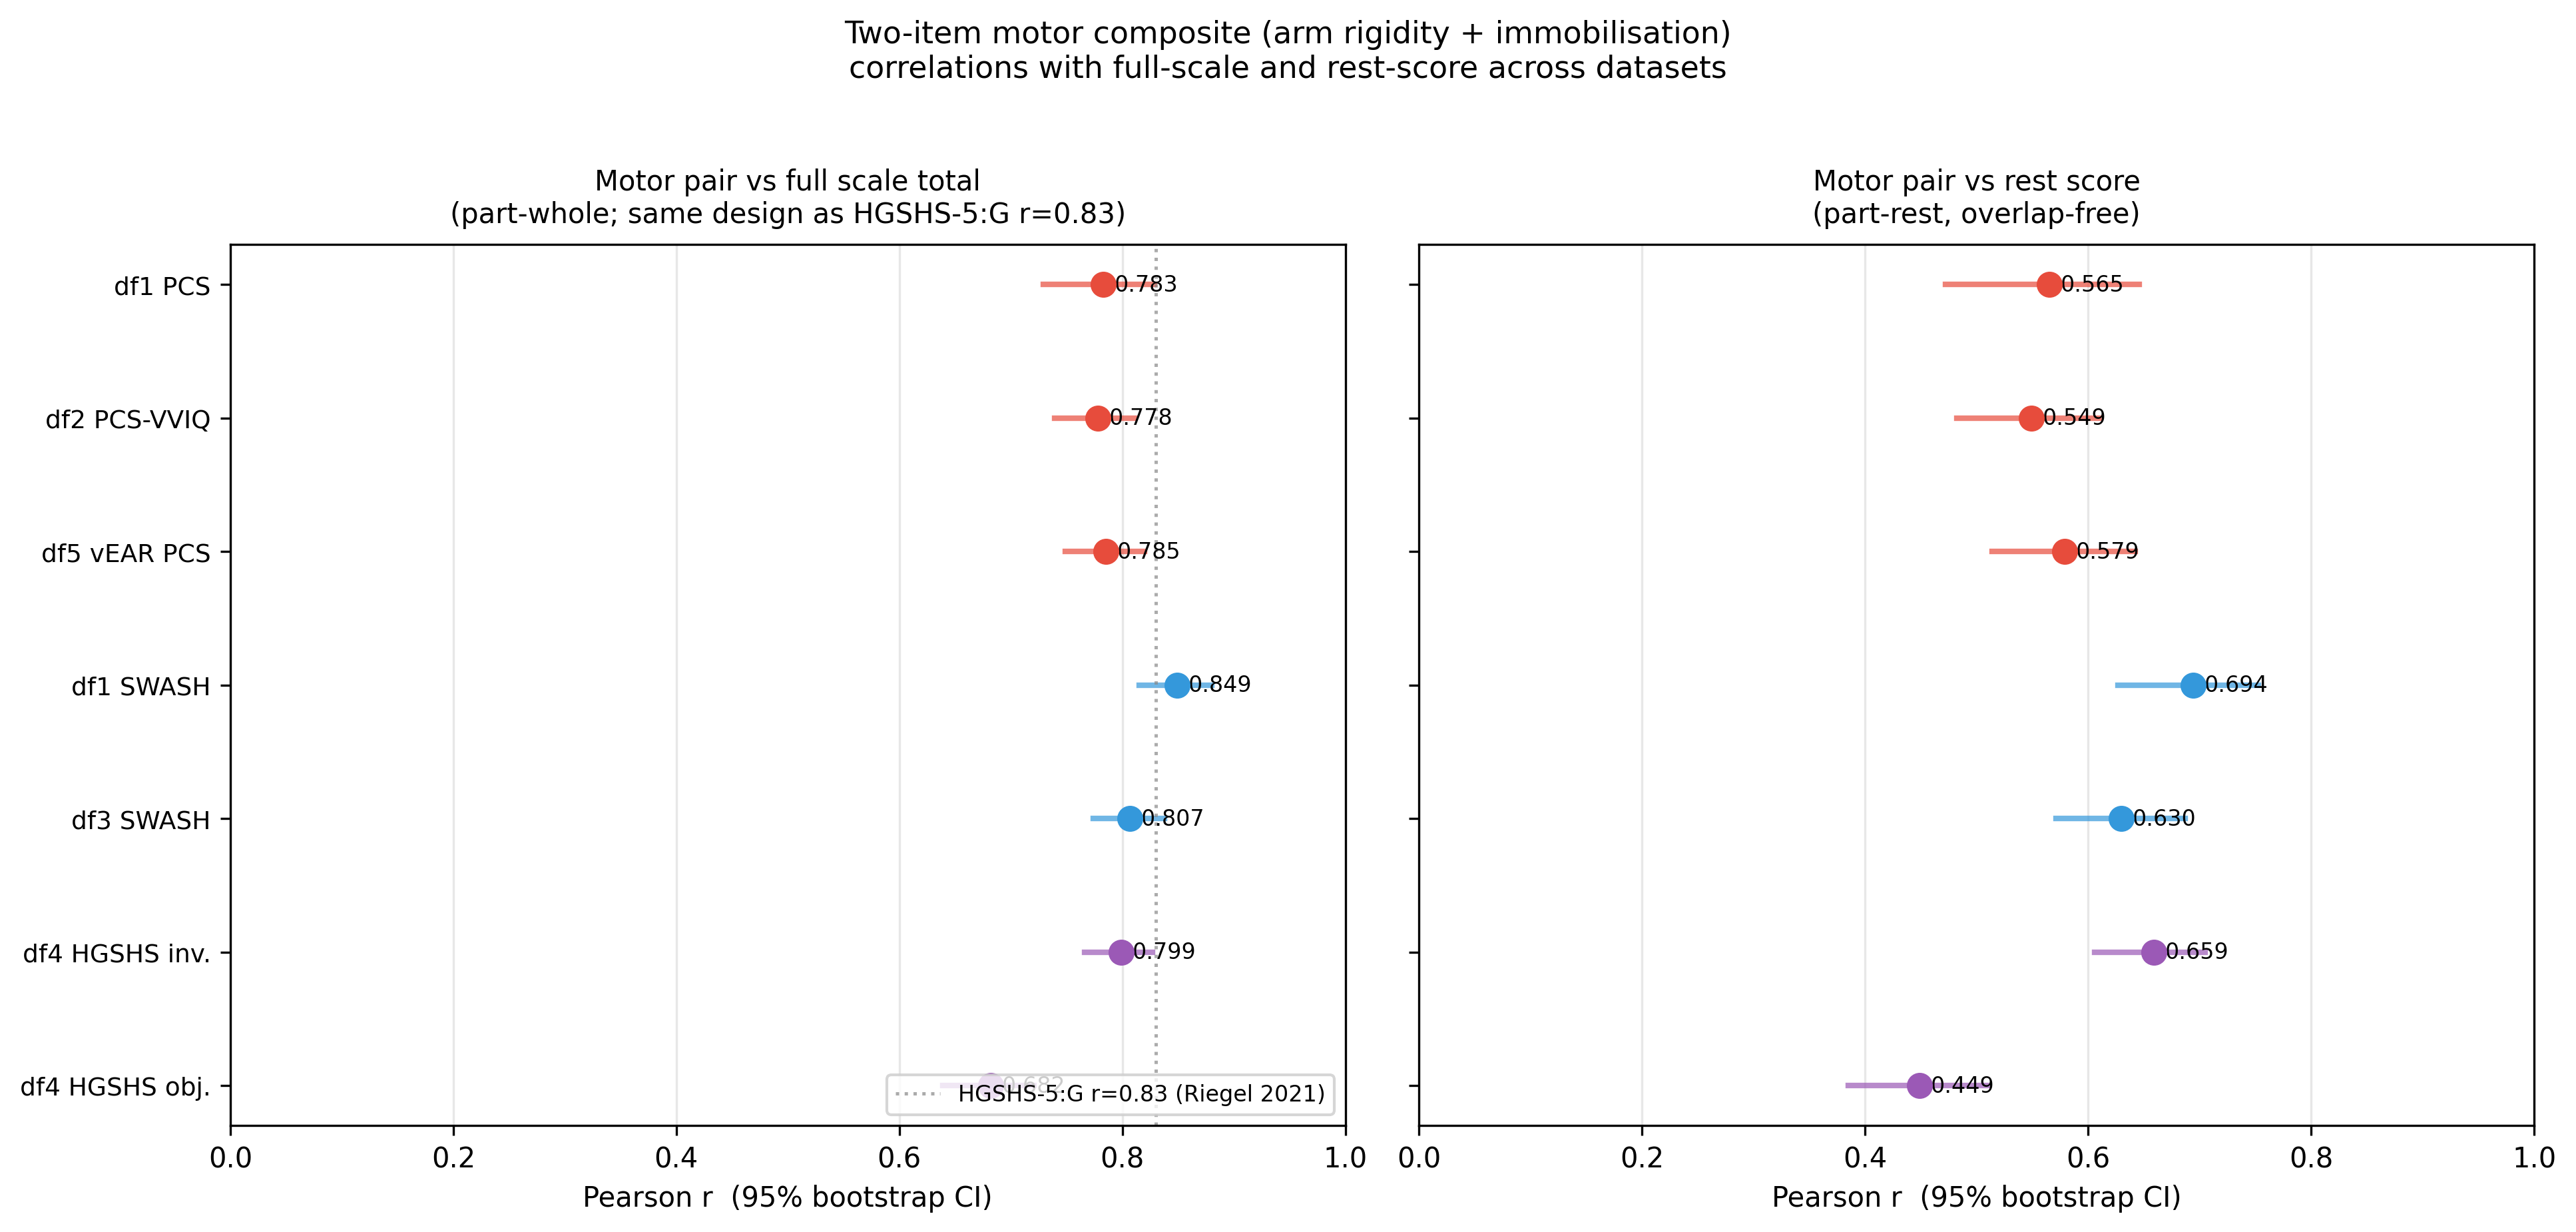
\includegraphics[width=\textwidth]{figures/fig1_forest_plot.png}
\caption{Forest plot: motor composite $r_{\text{full}}$ (left) and
  $r_{\text{rest}}$ (right) with 95\% CIs across datasets. Red\,=\,PCS,
  blue\,=\,SWASH, purple\,=\,HGSHS:A. Dotted line: HGSHS-5:G $r = 0.83$.}
\label{fig:forest}
\end{figure}

\subsection{Floor effects}

Figure~\ref{fig:floor} shows per-item means and floor rates. Music
hallucination and negative visual hallucination are near floor in every
dataset: 80--93\% at zero, means 0.14--0.43/5. The motor items sit near
mid-scale (means 2.0--3.2/5, floor rates 5--12\%). With near-universal zero scores, these items add little to between-person
variance on the total, which is therefore disproportionately shaped by the
items that retain between-person spread.
This is consistent with bifactor analysis of HGSHS:A \citep{zahedi2022bifactor}.

\begin{figure}[ht]
\centering
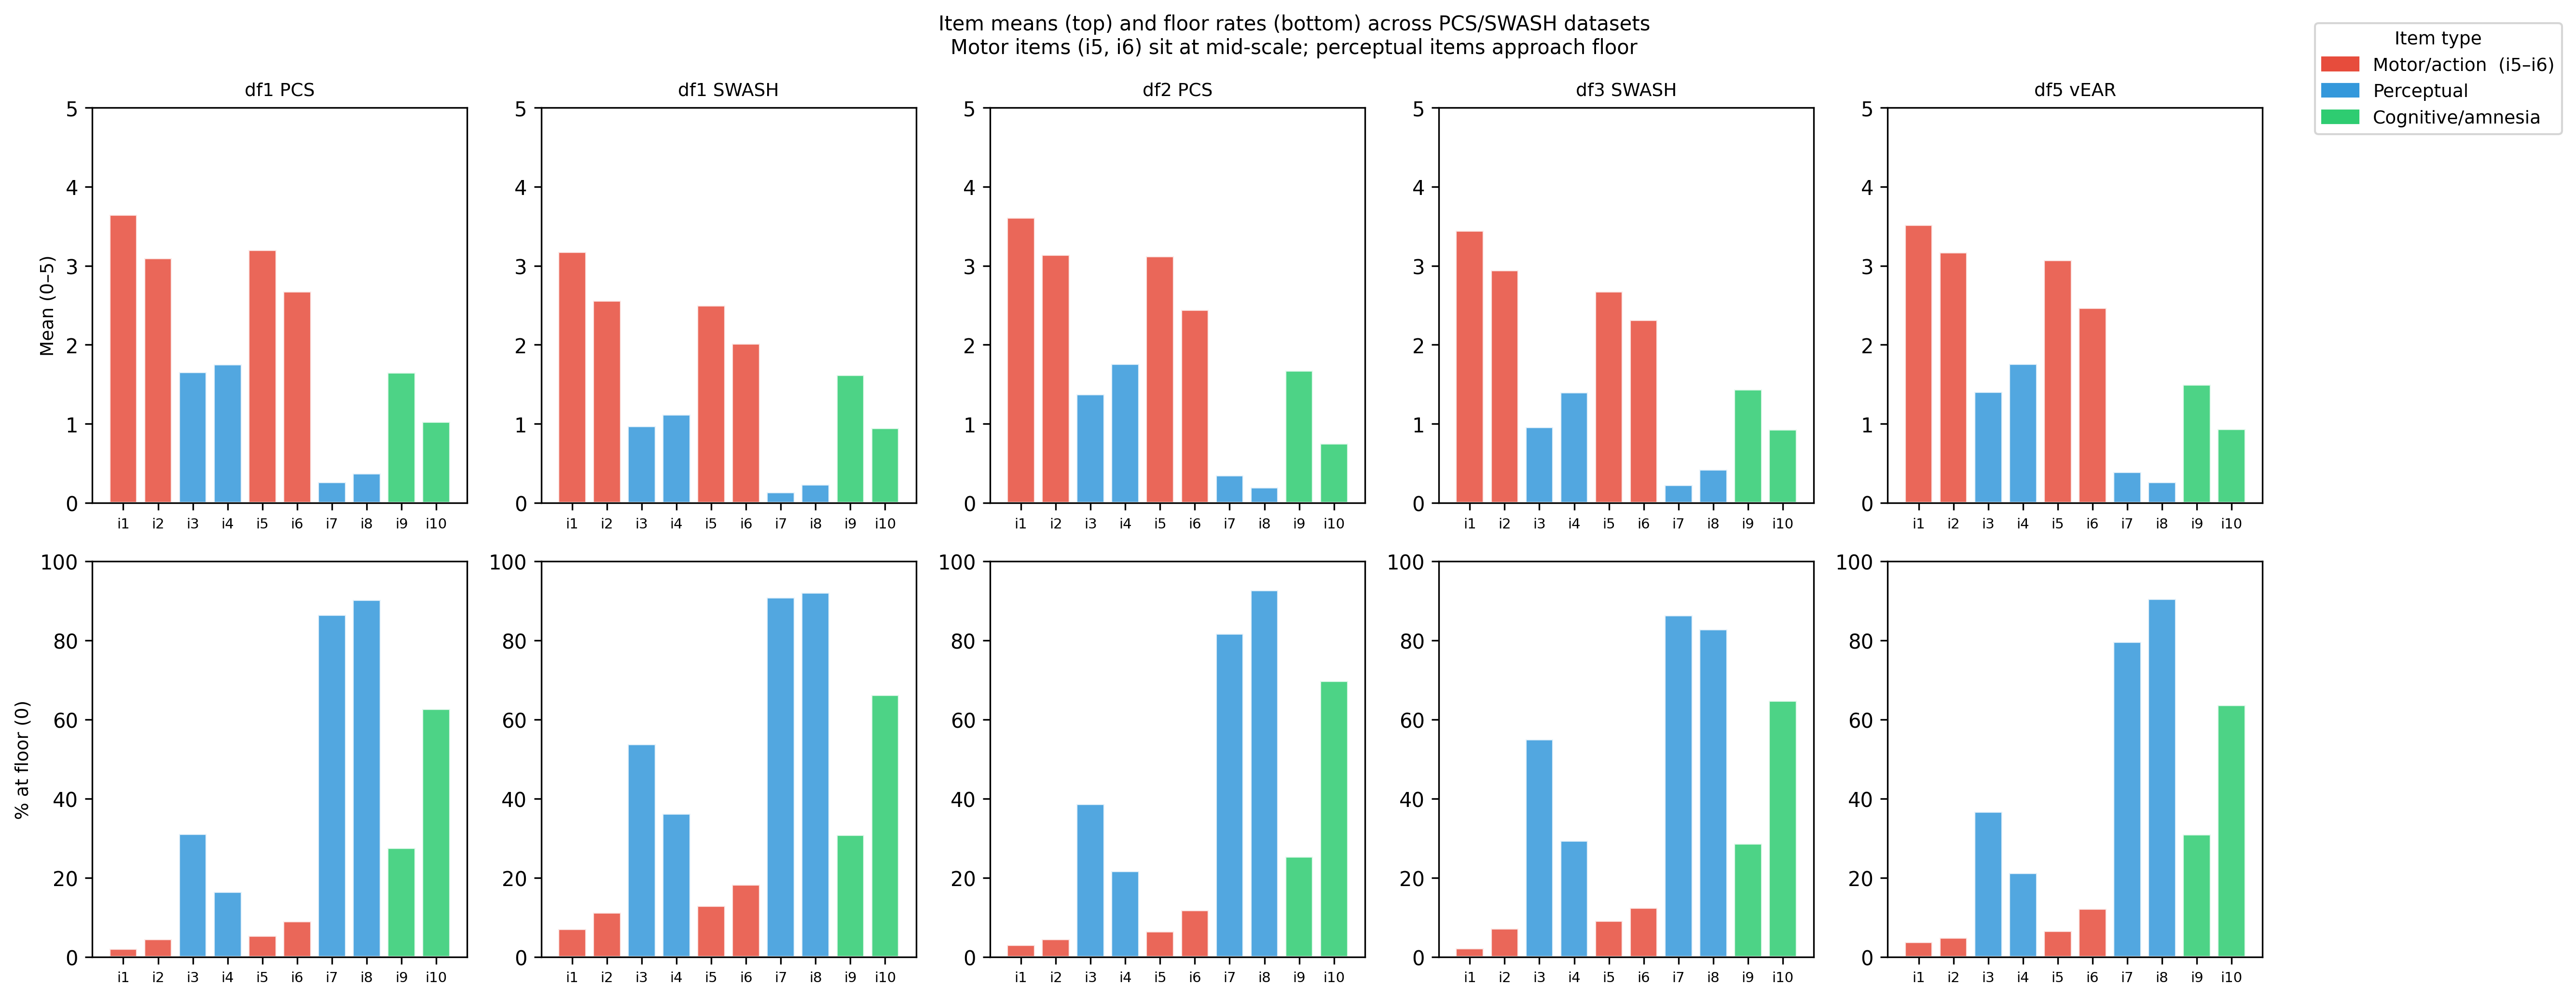
\includegraphics[width=\textwidth]{figures/fig3_item_floor.png}
\caption{Per-item means (top) and floor rates (bottom) across five
  intensity datasets. Red\,=\,motor items (i5, i6); blue\,=\,perceptual;
  green\,=\,cognitive/amnesia.}
\label{fig:floor}
\end{figure}

\subsection{External validity}

Table~\ref{tab:external} and Figure~\ref{fig:external} show correlations
with external criteria sharing no items with the PCS. The motor pair
retains 71--80\% of the full scale's correlation with vEAR and anomalous
experiences, the two criteria where both scales show nonzero signal. On
both, the non-motor rest score predicts outcomes slightly more strongly than
the motor pair (vEAR: $r_{\text{rest}} = 0.354$ vs.\ $r_{\text{motor}} =
0.297$; anomalous: $r_{\text{rest}} = 0.189$ vs.\ $r_{\text{motor}} =
0.155$); the rest score carries eight items to the pair's two. The motor
pair indexes the shared first component; the perceptual and cognitive items
carry domain-specific variance beyond it. Flow and DES
correlations are near-zero for both the motor pair and the full scale;
retention percentages for those criteria are not meaningful.

\begin{table}[ht]
\centering
\caption{External validity: motor pair vs.\ full scale (no item overlap).}
\label{tab:external}
\small
\begin{tabular}{lrrrrl}
\toprule
Criterion & $N$ & $r_{\text{motor}}$ & $r_{\text{rest}}$ & $r_{\text{full}}$ & Retained \\
\midrule
vEAR (video-rated)    & 452 & 0.297 & 0.354 & 0.372 & 80\% \\
Anomalous experiences & 497 & 0.155 & 0.189 & 0.202 & 77\% \\
Past-life experiences & 497 & 0.158 & 0.214 & 0.221 & 71\% \\
Flow (combined)       & 432 & 0.109 & 0.131 & 0.139 & 78\%$^\dagger$ \\
DES dissociation      & 559 & 0.100 & 0.092 & 0.107 & ---$^\dagger$ \\
\bottomrule
\multicolumn{6}{l}{\parbox{11cm}{$^\dagger$ Both values near zero; retention percentage uninformative.}}\\
\end{tabular}
\end{table}

\begin{figure}[ht]
\centering
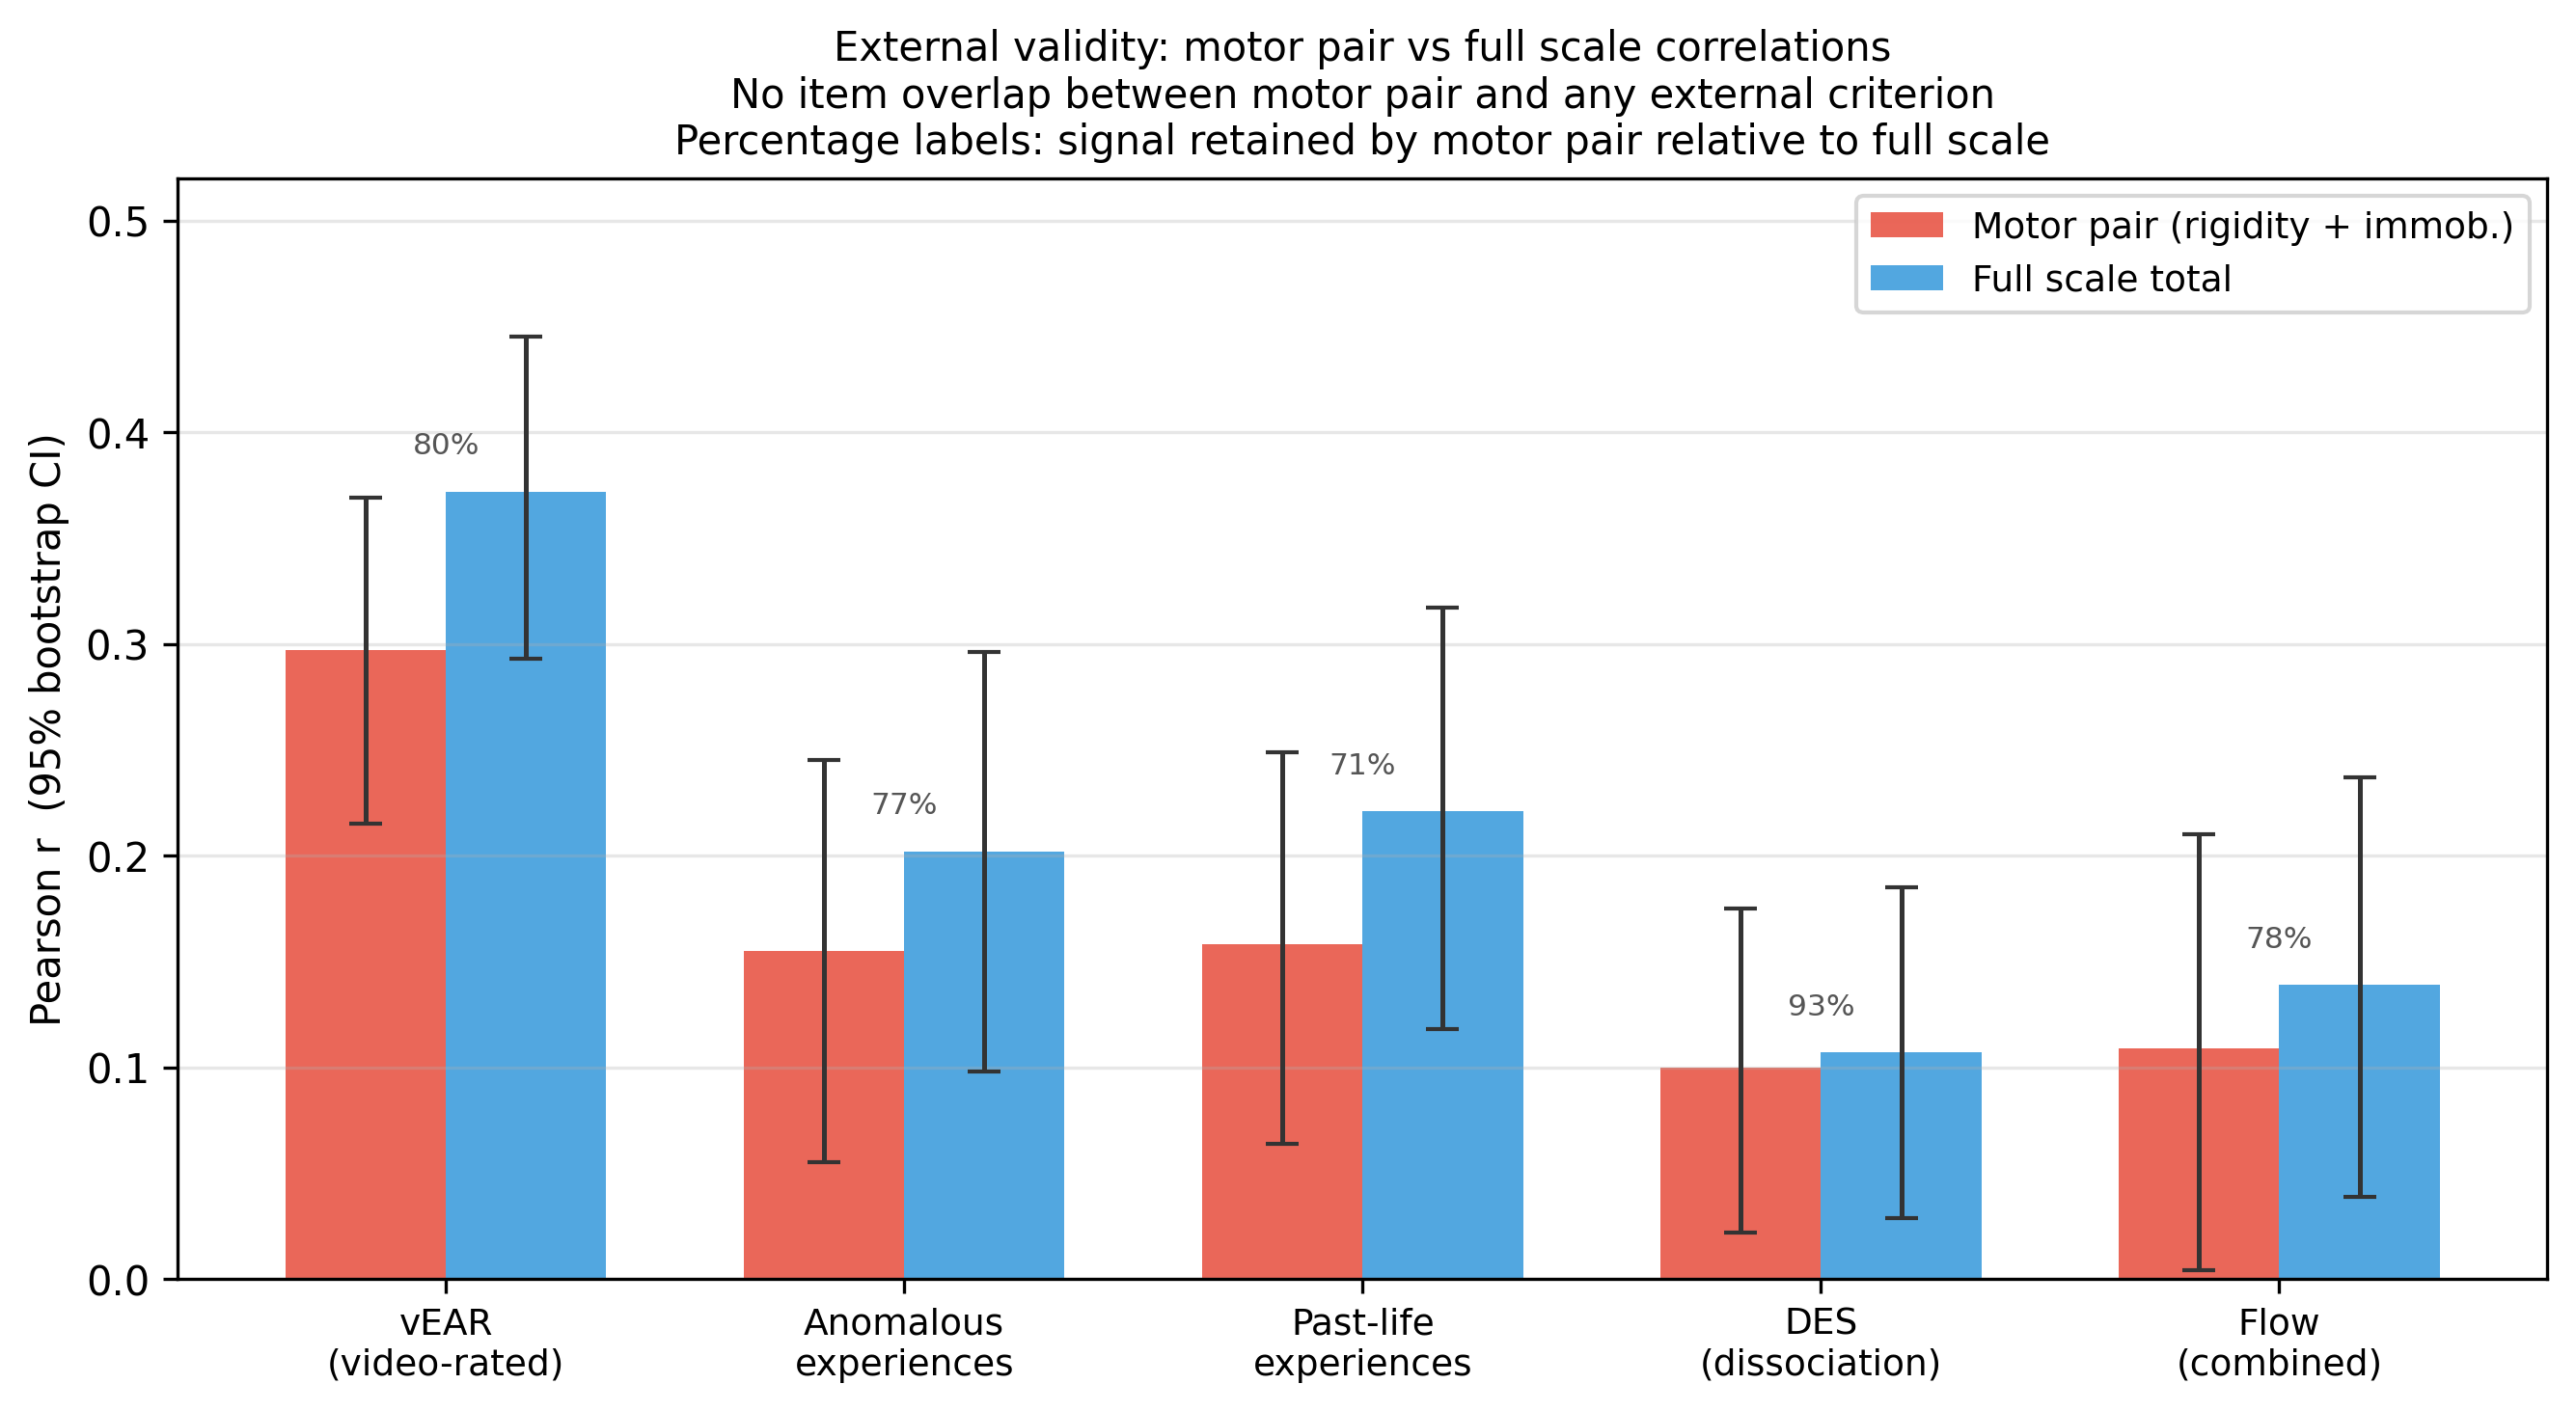
\includegraphics[width=0.9\textwidth]{figures/fig5_external_validity.png}
\caption{Motor pair (red) vs.\ full scale (blue) with external criteria.
  Error bars: 95\% bootstrap CIs. Labels: \% of full-scale $r$ retained.}
\label{fig:external}
\end{figure}

\subsection{Classification}

Table~\ref{tab:classification} shows three-group weighted $\kappa$ and AUC
for top-third classification. Against the full total, PCS reaches
$\kappa_w = 0.50$--$0.55$ and SWASH/HGSHS:A involuntariness reaches
$\kappa_w = 0.65$. The overlap-free rest-score criterion produces lower
values---PCS 0.29--0.34, SWASH 0.45--0.46, HGSHS:A involuntariness
0.52---quantifying the portion of agreement attributable to shared items.
AUC ranges from 0.83--0.86 (PCS) to 0.89--0.91 (SWASH/HGSHS:A
involuntariness). Binary cutoff sweeps show high specificity (0.87--0.99)
across the full 8--33\% range; sensitivity is modest at tight cutoffs.

\begin{table}[ht]
\centering
\caption{Classification: weighted $\kappa$ and AUC.}
\label{tab:classification}
\small
\begin{tabular}{lrrrrrr}
\toprule
 & & \multicolumn{2}{c}{Full total} & \multicolumn{2}{c}{Rest score} & \\
\cmidrule(lr){3-4}\cmidrule(lr){5-6}
Sample & $N$ & $\kappa_w$ & $\kappa_u$ & $\kappa_w$ & $\kappa_u$ & AUC \\
\midrule
Norms-PCS      & 244 & 0.548 & 0.446 & 0.325 & 0.262 & 0.829 \\
PCS-VVIQ       & 508 & 0.504 & 0.400 & 0.294 & 0.203 & 0.852 \\
vEAR-PCS       & 452 & 0.522 & 0.410 & 0.335 & 0.240 & 0.858 \\
\midrule
Norms-SWASH    & 240 & 0.657 & 0.550 & 0.459 & 0.355 & 0.905 \\
SWASH-val      & 418 & 0.652 & 0.547 & 0.448 & 0.363 & 0.896 \\
\midrule
HGSHS:A (inv.) & 584 & 0.651 & 0.563 & 0.522 & 0.442 & 0.893 \\
HGSHS:A (obj.) & 584 & 0.554 & 0.459 & 0.347 & 0.267 & 0.841 \\
\midrule
\textit{HGSHS-5:G (prior short form)} & --- & \textit{$\approx$0.58} & & & & \\
\bottomrule
\multicolumn{7}{l}{\parbox{12cm}{\textit{Note.} AUC: top-third on full total. Rest score: non-motor items. HGSHS-5:G: \citet{riegel2021hgshs5g, zech2024hgshs5g}.}}\\
\end{tabular}
\end{table}

\begin{figure}[ht]
\centering
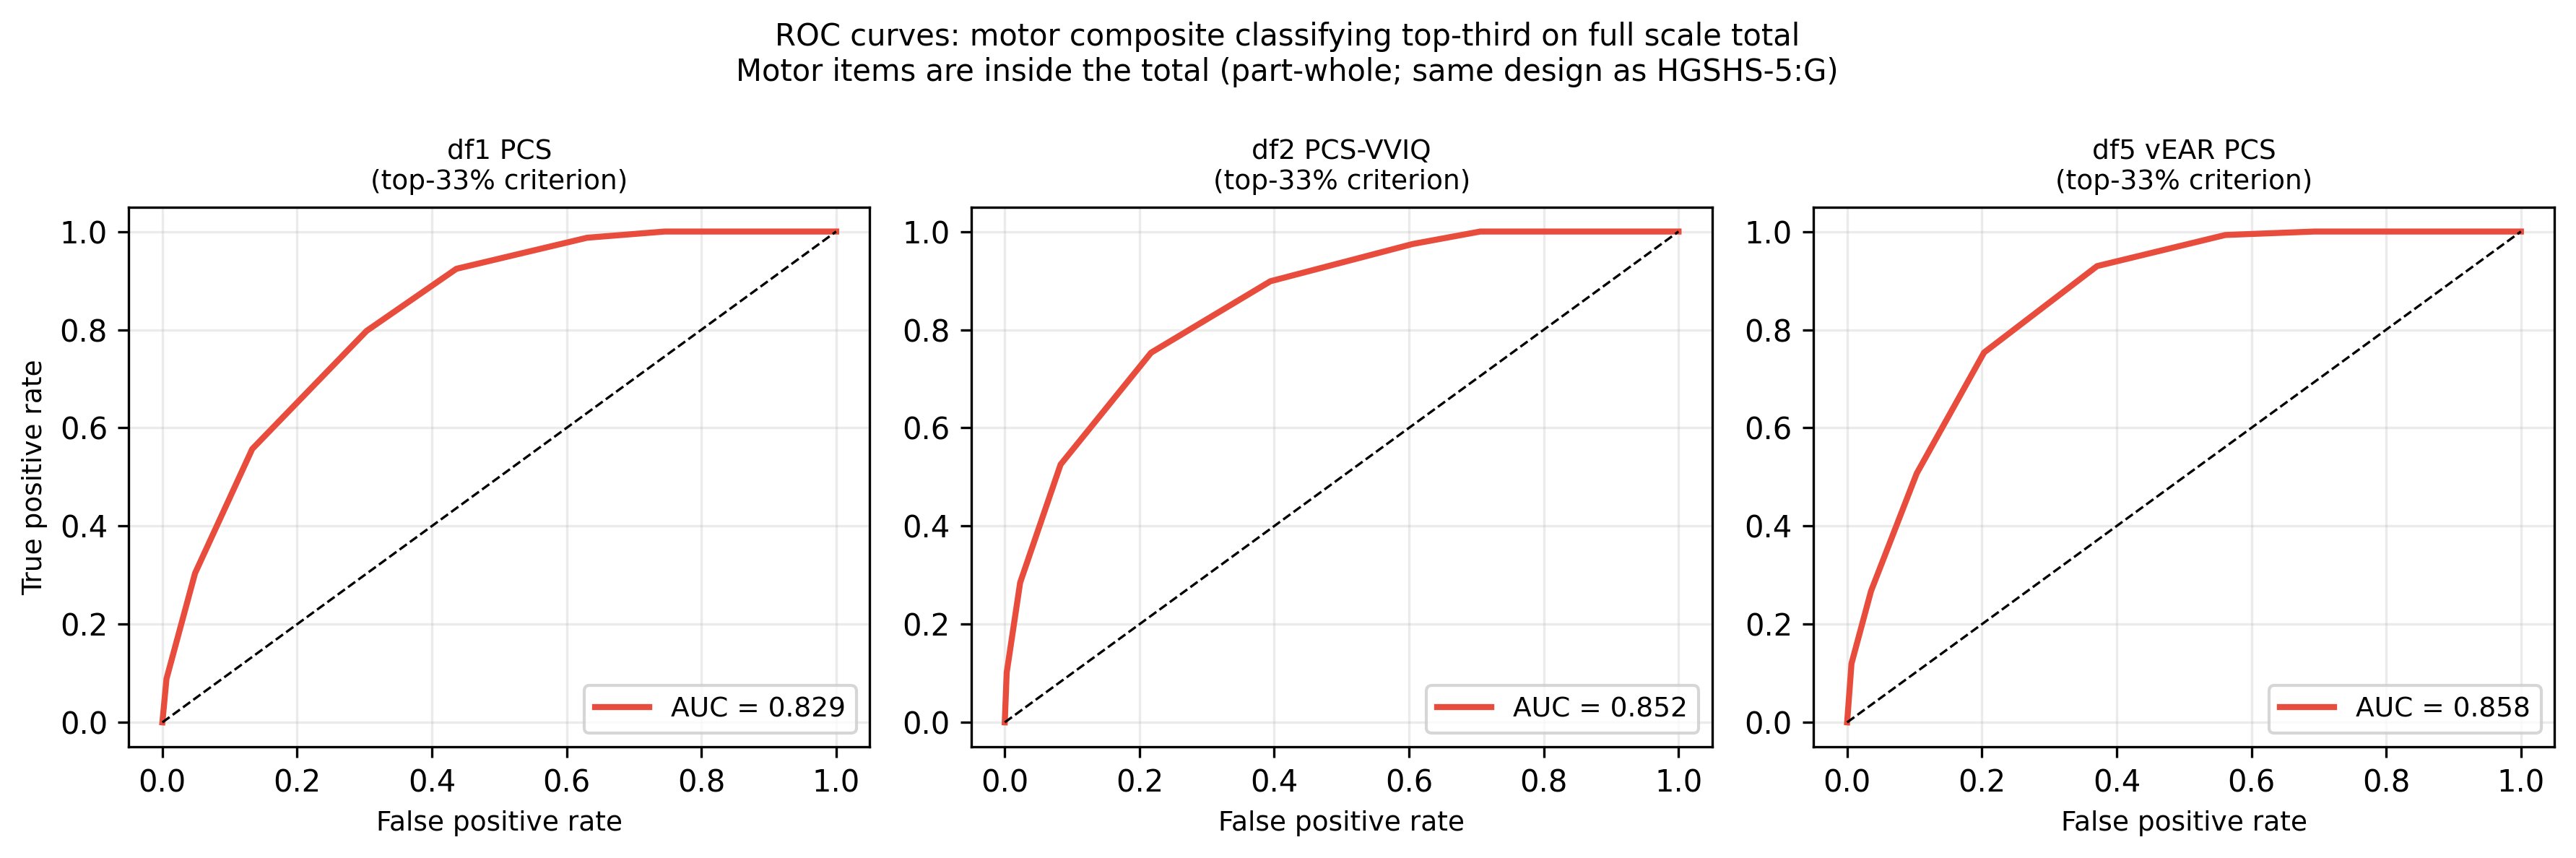
\includegraphics[width=\textwidth]{figures/fig4_roc_primary.png}
\caption{ROC curves: motor composite classifying top-third on full total,
  three PCS datasets. AUC = 0.829, 0.852, 0.858.}
\label{fig:roc}
\end{figure}

\subsection{All-pairs analysis}

Figure~\ref{fig:allpairs} shows where the motor pair falls among all 45
possible two-item combinations per dataset. By $r_{\text{full}}$, the
motor pair ranks first or second in all three PCS datasets and fourth in
the Norms-SWASH dataset; in the SWASH validation dataset it ranks 13th,
where the top pair is taste + arm rigidity ($r_{\text{full}} = 0.845$).
The $r_{\text{rest}}$ ranking is weaker---the motor pair drops to ranks 2,
9, 11, 8, and 23 across the five datasets. A motor item appears in the top
pair in every dataset; perceptual floor items never do.

\begin{figure}[ht]
\centering
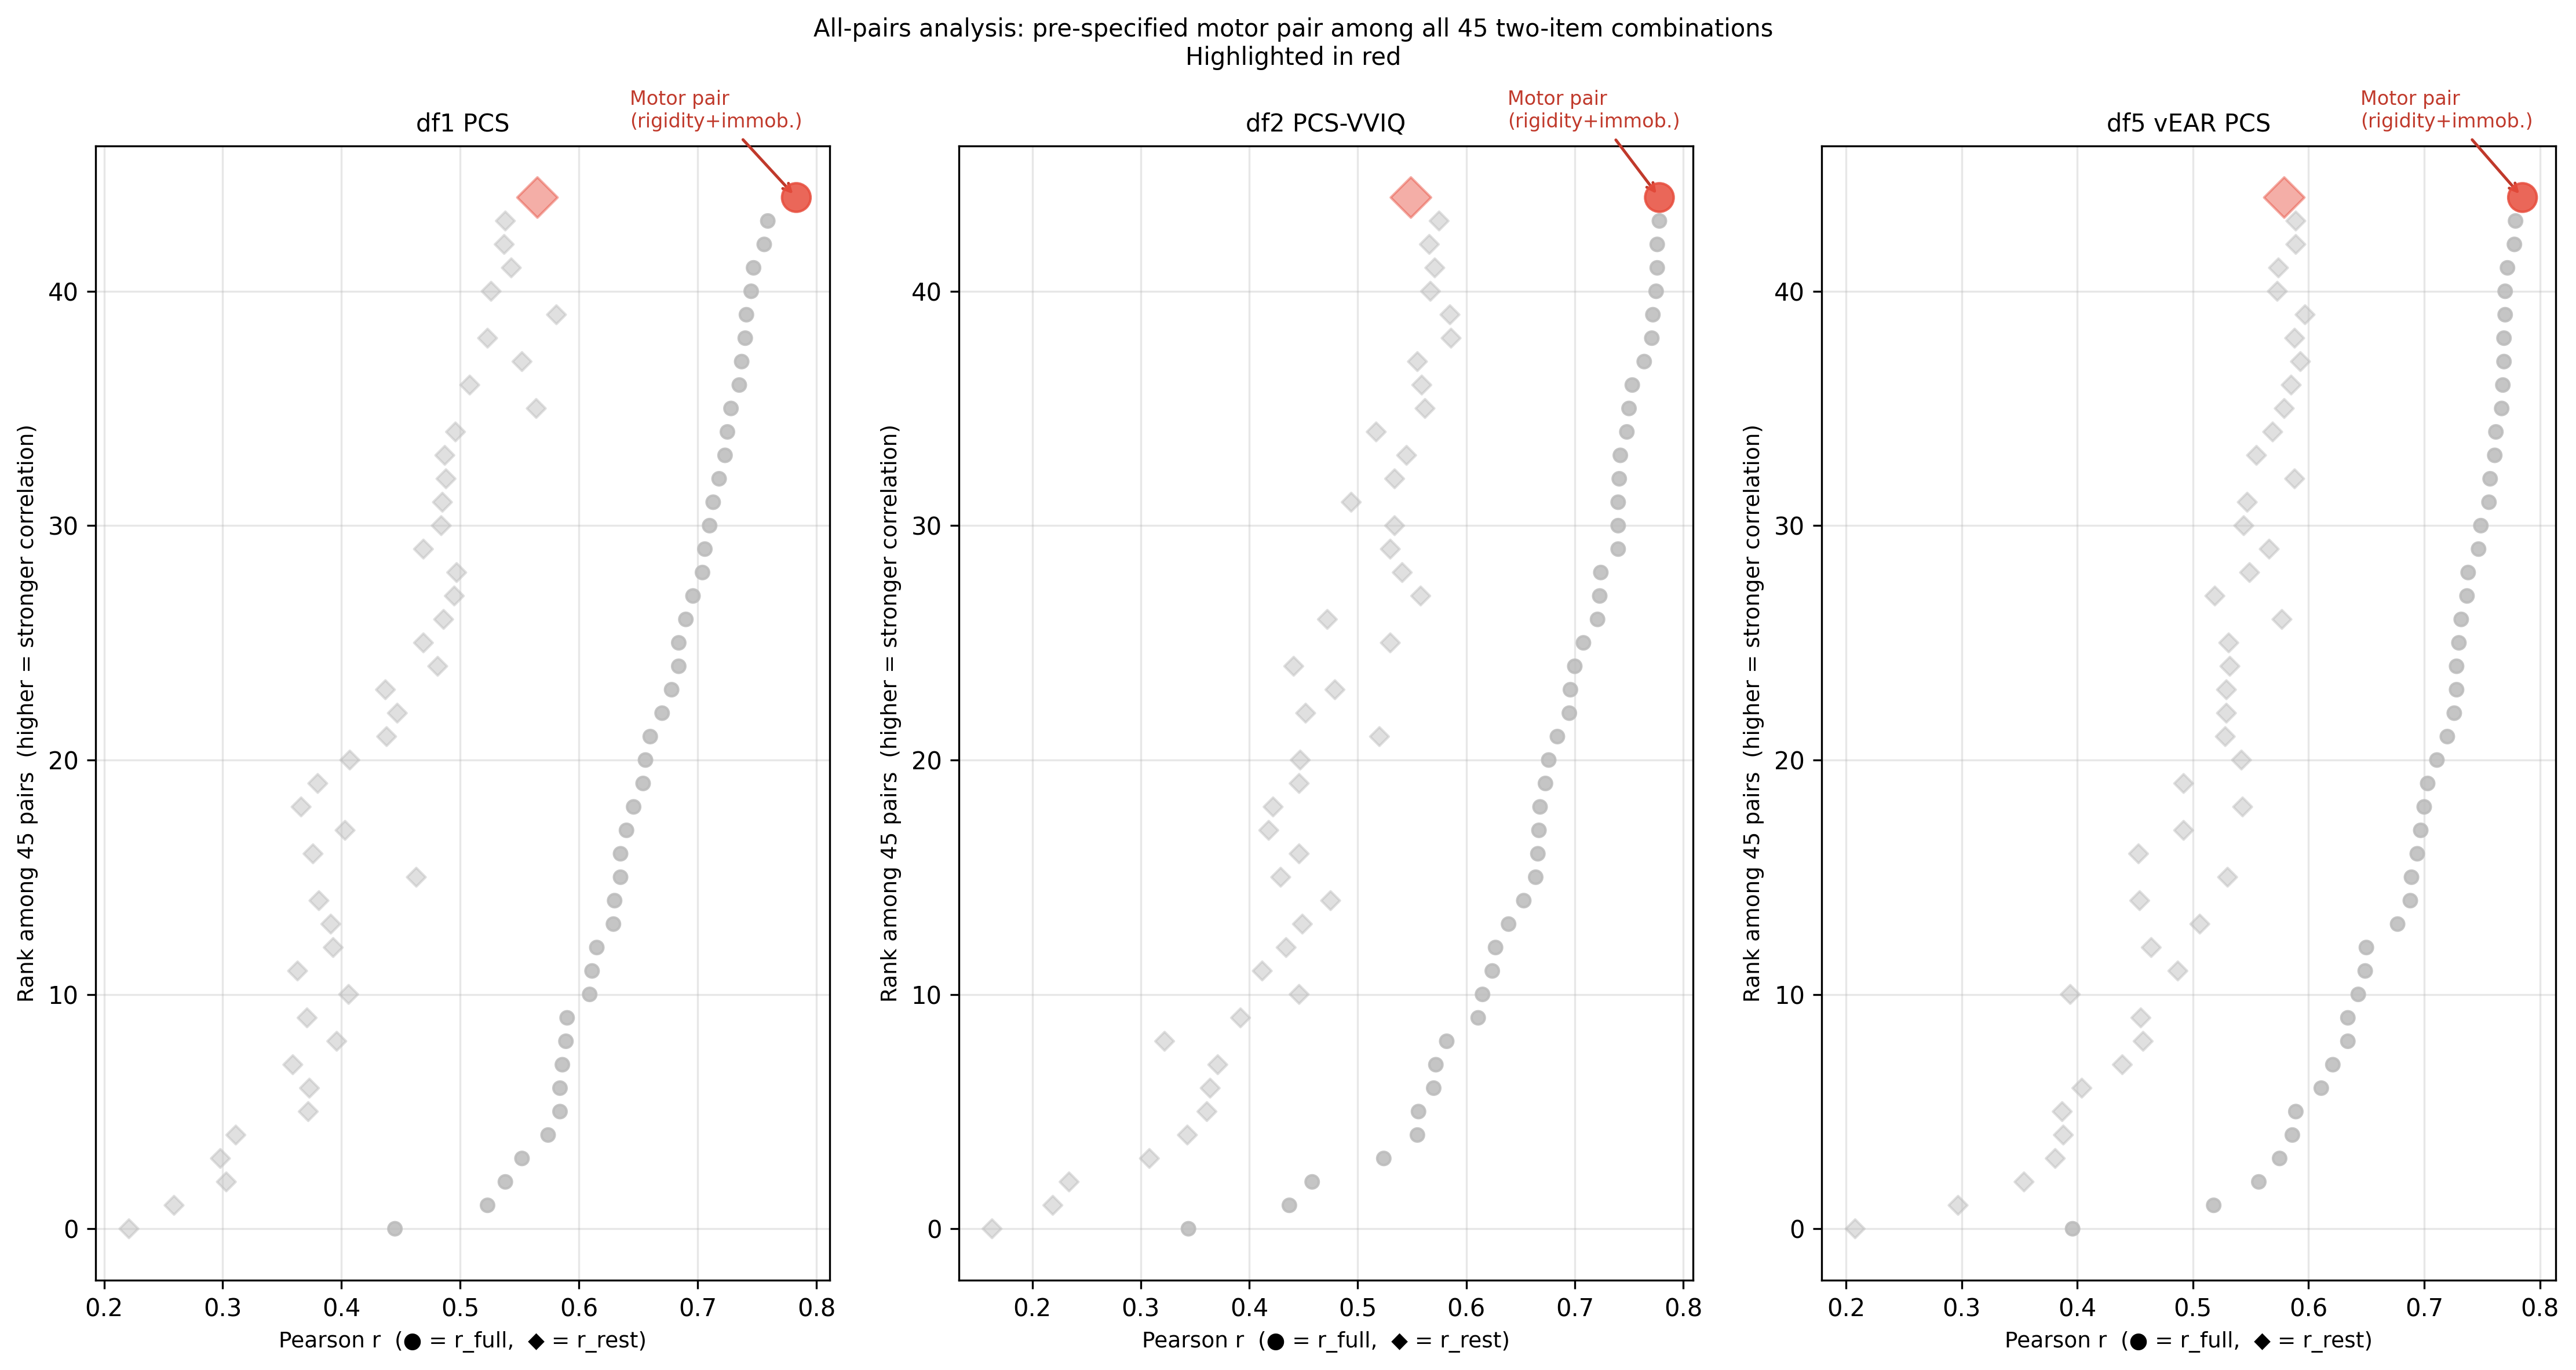
\includegraphics[width=\textwidth]{figures/fig2_all_pairs_rank.png}
\caption{All 45 two-item combinations ranked by $r_{\text{full}}$
  (circles) and $r_{\text{rest}}$ (diamonds) across three PCS datasets.
  Motor pair in red.}
\label{fig:allpairs}
\end{figure}

\subsection{Temporal stability}

Embedded motor-pair test-retest: $r = 0.338$ ($n = 61$, PCS; full scale:
$r = 0.523$; SWASH: $r = 0.497$). Overlap-free motor-T1 to rest-T2:
$r = 0.222$ (PCS, ns). Both figures are from embedded administrations
within the full ten-item procedure; standalone two-item retest stability
is unknown and may differ in either direction.


% ============================================================
\section{Discussion}

Among all 45 two-item subsets of the established ten-item pool, the motor
pair is the top-ranked or near-top-ranked pair in every dataset, with a
motor item in the leading pair regardless of scale or context; the optimality
claim is bounded to this comparison class. The structure---variance
concentrating in motor-challenge items---holds across non-hypnotic (PCS),
hypnotic (SWASH), and classic group (HGSHS:A) administration and across
intensity and involuntariness axes. The magnitude of that concentration
differs by context: the randomised Norms comparison, where the same pool was
assigned to PCS or SWASH, establishes that stronger motor-pair coupling under
induction reflects the administered context rather than cohort composition
($r_{\text{full}}$: $p = .029$; $r_{\text{rest}}$: $p = .018$).

Floor effects explain the high $r_{\text{full}}$ values. In unselected
samples, music hallucination and negative visual hallucination score zero
for the great majority of participants; with near-zero variance they
contribute little to between-person rank-ordering on the total, which is
therefore dominated by the motor items. The near-floor perceptual items are
difficult suggestions carrying domain-specific variance that the two-item
screen gives up; the rest score, with eight items to the pair's two, also
carries a reliability advantage that accounts for part of its slightly
higher external signal.

High specificity (0.87--0.99 across the binary sweep) means that high
motor-pair scores have a low false-positive rate for top-third status; modest
sensitivity at tight cutoffs means some true high responders will not be
flagged. That trade-off is appropriate for first-pass triage, not final
selection.

Four limits bound the interpretation. These are embedded administrations:
standalone two-item performance is untested. Floor concentration is
sample-dependent: in enriched high-responding samples the proxy advantage
will shrink. HGSHS:A indexes involuntariness and objective pass/fail, not
subjective intensity; its results are not directly comparable with the PCS
and SWASH findings. All analyses are secondary reanalysis of open data; no
new data were collected.


% ============================================================
\section*{Open Science Statement}

\textbf{Data.} All datasets are on OSF:
Norms sample: \url{osf.io/et85n};
PCS-VVIQ sample: \url{osf.io/aeyhw};
SWASH validation sample: \url{osf.io/wujk8};
HGSHS:A sample: \url{osf.io/jfmc4};
vEAR-PCS sample: \url{osf.io/a2skp};
external criteria: \url{osf.io/u5wjy}.

\textbf{Code.} \texttt{analysis.ipynb}, \texttt{lib\_data.py}, and
analysis scripts \texttt{a01}--\texttt{a08} at
\url{https://github.com/Wordweaver-EH/Hypnoscales}.

\textbf{Author contributions (CRediT).} [To be completed at submission.]

% ============================================================
\clearpage
\section*{Supplementary Materials}

\subsection*{S1. Analysis code}

All analysis code is available at
\url{https://github.com/Wordweaver-EH/Hypnoscales}.
The pipeline consists of the following files:

\begin{itemize}
  \item \texttt{lib\_data.py} --- Shared data-loading, canonical scoring,
    exclusion logic, motor-pair column mappings, and bootstrap CI functions.
    All analysis scripts import from this file; nothing is hard-coded
    elsewhere.
  \item \texttt{a01\_descriptives.py} --- Per-item means, SDs, floor and
    ceiling rates, and dataset summary table
    (\texttt{table\_item\_descriptives.csv},
    \texttt{table\_dataset\_summary.csv}).
  \item \texttt{a02\_convergence.py} --- Motor composite correlations
    ($r_{\text{full}}$, $r_{\text{rest}}$, Spearman-Brown reliability) with
    bootstrap CIs and Fisher $r$-to-$z$ context comparisons
    (\texttt{table\_main\_convergence.csv}).
  \item \texttt{a03\_retest.py} --- Test-retest correlations for the motor
    pair, full scale, and overlap-free motor-T1 to rest-T2
    (\texttt{table\_test\_retest.csv}).
  \item \texttt{a04\_classification.py} --- Weighted Cohen's $\kappa$
    (tertile), AUC, and binary cutoff sweep for sensitivity, specificity,
    PPV, and NPV (\texttt{table\_classification.csv}).
  \item \texttt{a05\_all\_pairs.py} --- $r_{\text{full}}$ and
    $r_{\text{rest}}$ for all $\binom{10}{2} = 45$ two-item combinations in
    the PCS/SWASH-style 10-item samples
    (\texttt{table\_all\_pairs.csv}).
  \item \texttt{a06\_external.py} --- Motor pair and full-scale correlations
    with five external criteria (no item overlap)
    (\texttt{table\_external\_validity.csv}).
  \item \texttt{a07\_sensitivity.py} --- Sensitivity checks: itemwise
    z-scored composites, listwise deletion, alternative cutoffs
    (\texttt{table\_sensitivity.csv}).
  \item \texttt{a08\_figures.py} --- All publication figures (Figures 1--5).
  \item \texttt{analysis.ipynb} --- Self-contained Jupyter notebook that
    reproduces the full pipeline inline, with inline narrative.
\end{itemize}

\subsection*{S2. Source datasets}

\begin{itemize}
  \item \textbf{Norms sample} (PCS + SWASH, between-subjects):
    \url{osf.io/et85n}. \citet{lush2021pcs}.
  \item \textbf{PCS-VVIQ sample}:
    \url{osf.io/aeyhw}. \citet{lush2021pcs}.
  \item \textbf{SWASH validation sample}:
    \url{osf.io/wujk8}. \citet{lush2018swash}.
  \item \textbf{HGSHS:A sample}:
    \url{osf.io/jfmc4}. \citet{acunzo2021standardized}.
  \item \textbf{vEAR-PCS sample} (external validity, convergence):
    \url{osf.io/a2skp}.
  \item \textbf{External criteria} (anomalous experiences, flow, DES,
    past-life, vEAR behavioural ratings):
    \url{osf.io/u5wjy}.
\end{itemize}

% ============================================================
\bibliographystyle{apalike}
\bibliography{references}

\end{document}
